%!TEX root = ../../dimensions-2016-game-book.tex

\definecolor{darkGreen}{RGB}{20,100,1}

\phChapterWorksheet{A Dicey Situation}{Main Puzzle 2}

A standard six-sided die has a \textbf{planar unfolding} of this form,
  created by cutting along some of the edges and flattening the faces into
  a plane:

  \vfill

\begin{center}
 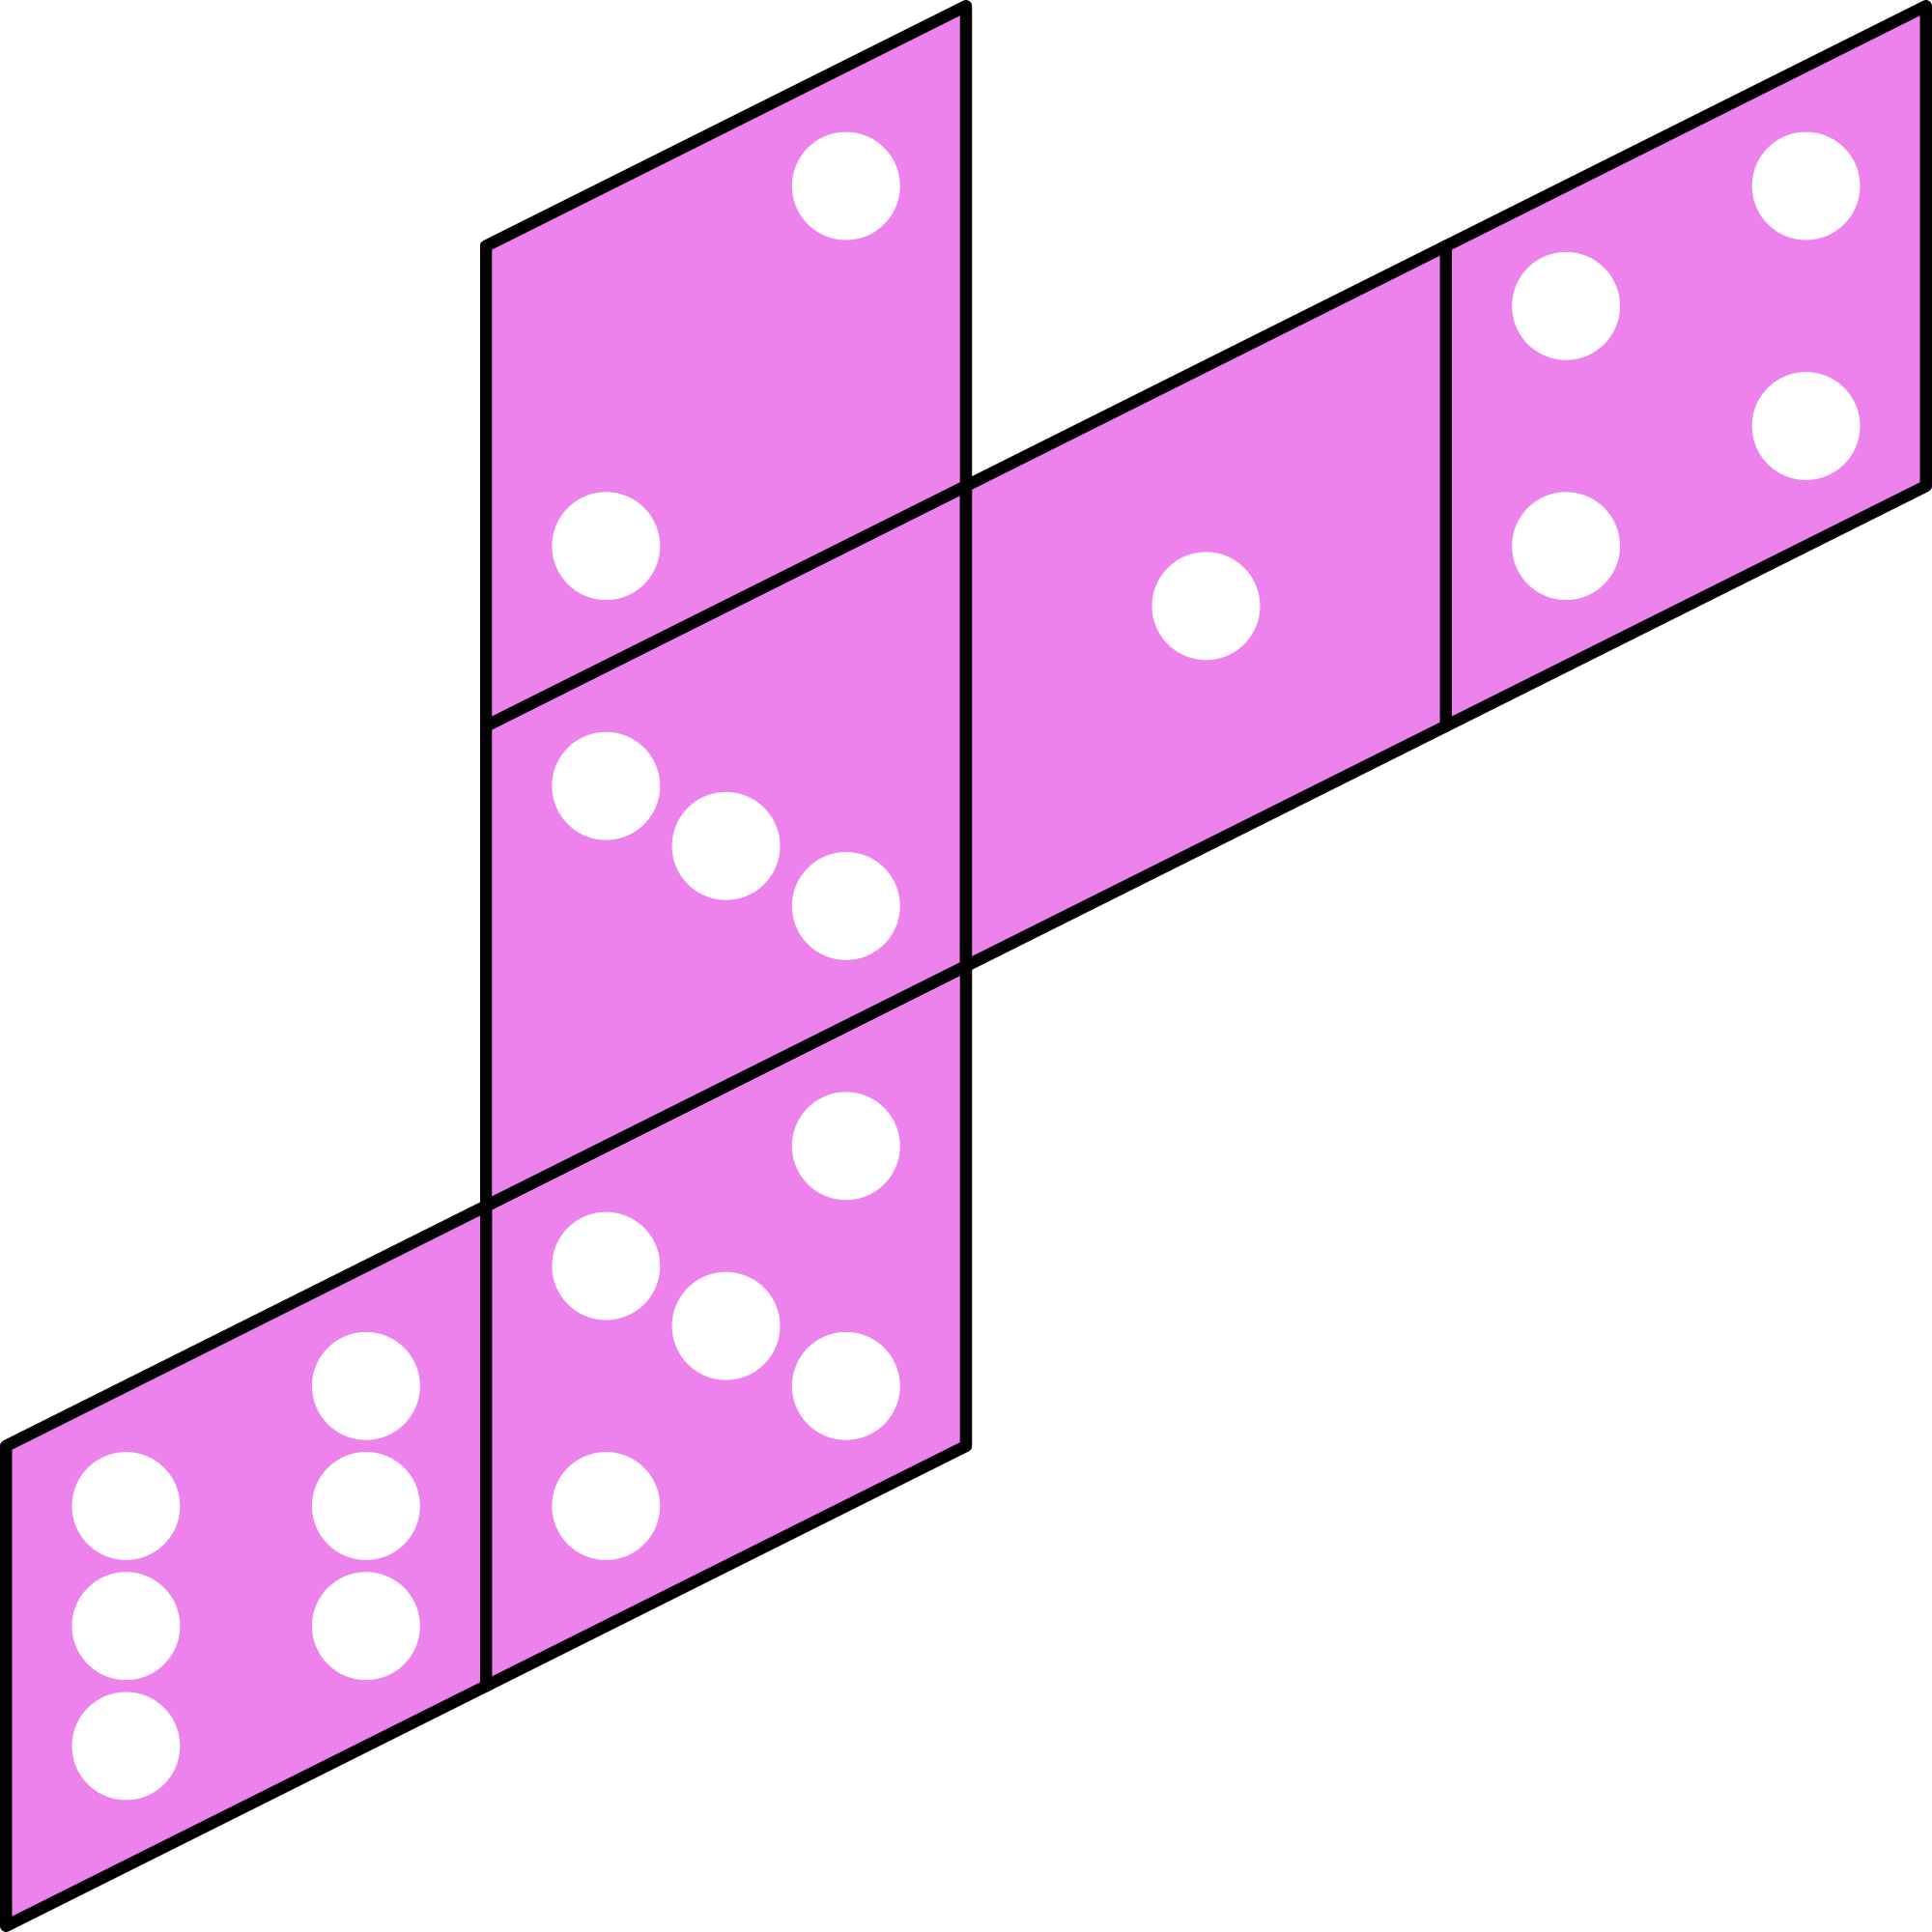
\includegraphics[width=0.3\linewidth]{diceExample.png}
\end{center}

  \vfill

  In the following images, three different-colored standard dice have been
  moved on an $8\times 8$ board:
    \textcolor{red}{red},
    \textcolor{darkGreen}{green}, and
    \textcolor{blue}{blue}.
  Two of the dice in each figure are moved by ``rolling'' the dice carefully
  from square to square as in the following image.

  \vfill

\begin{center}
  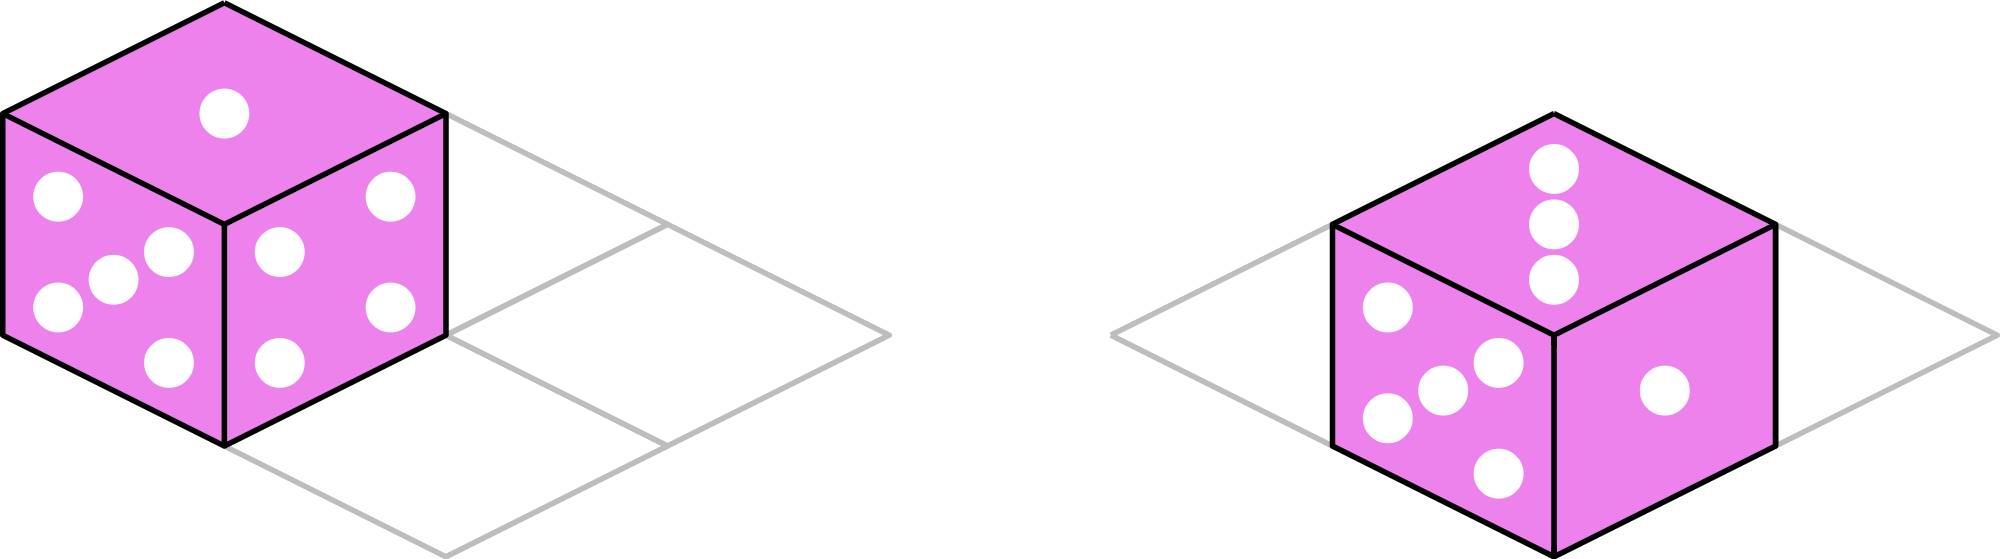
\includegraphics[width=0.5\linewidth]{diceLegal.png}
\end{center}

  \vfill

  However, the third color die in each image was simply picked up
  and placed at its new location. A clue to the location of an
  EXTRA Puzzle may
  be obtained by concatenating the strings of letters associated with this
  third die from each figure. (Look out: the images don't appear in the
  same order as the resulting message.)

  Relay the decrypted message to Game HQ for \(100\) points!

  \vfill

  \newpage



  \begin{center}
    \begin{tabular}{c}
      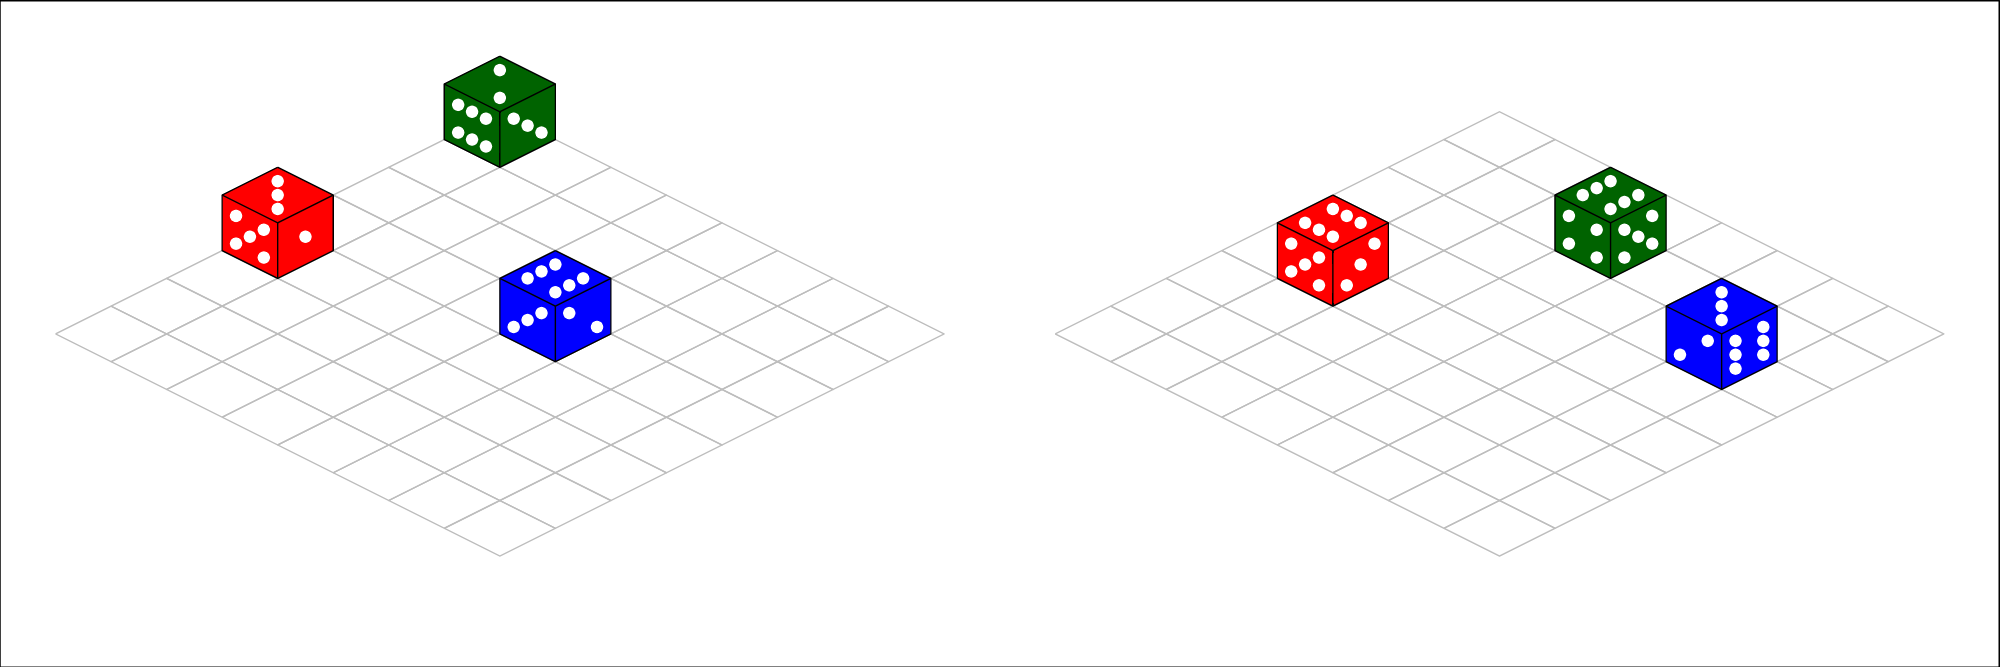
\includegraphics[width=0.8\linewidth]{diceBlue02.png}
      \\
      \textcolor{red}{JUS} |
      \textcolor{darkGreen}{AST} |
      \textcolor{blue}{GIS}
    \end{tabular}
  \end{center}


  \vfill


  \begin{center}
    \begin{tabular}{c}
      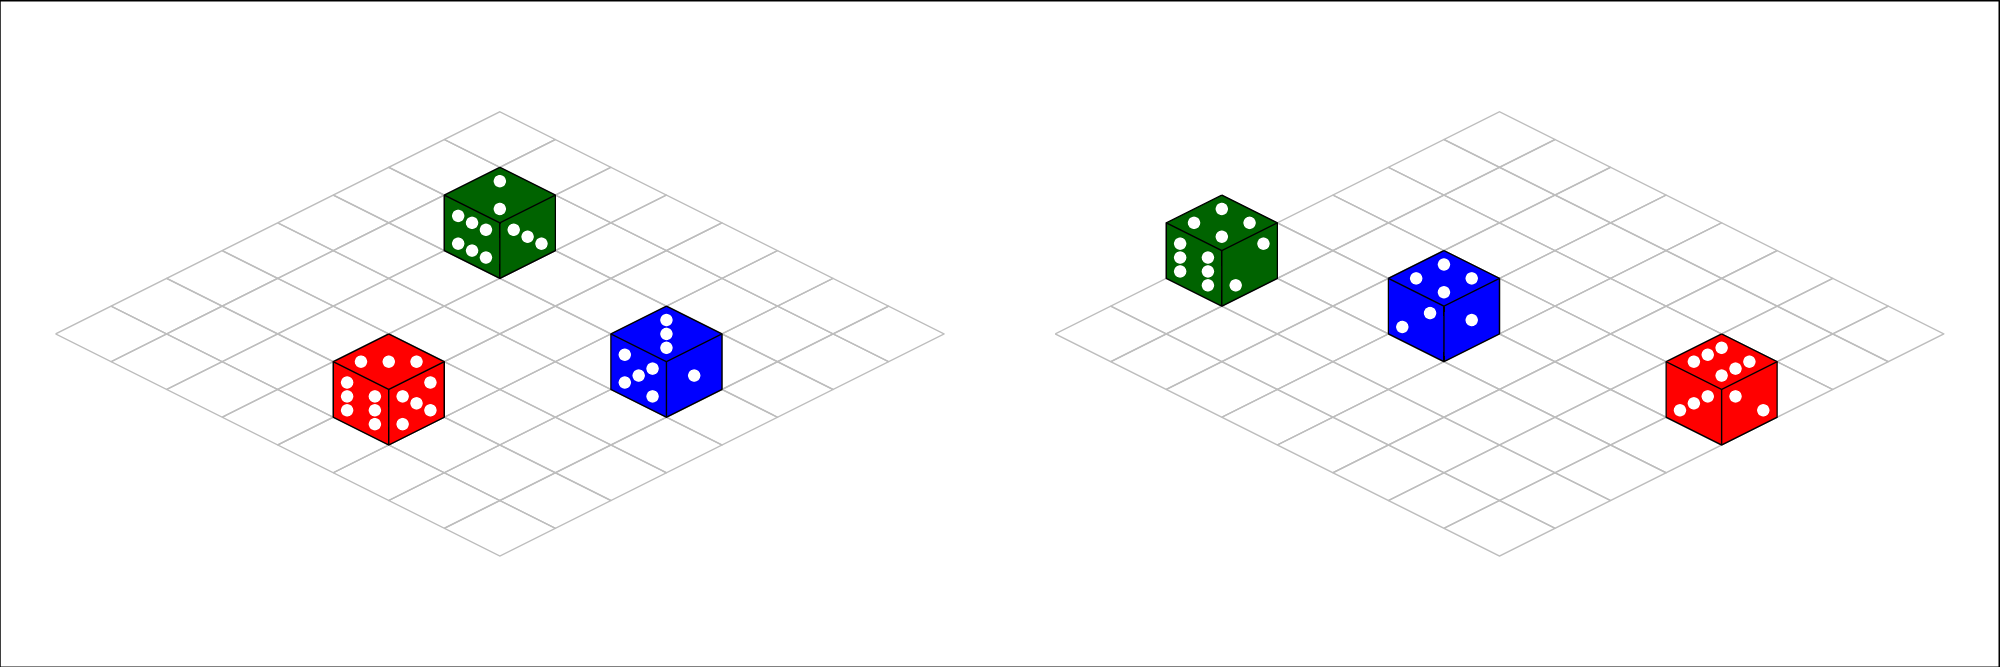
\includegraphics[width=0.8\linewidth]{diceRed03.png}
      \\
      \textcolor{red}{NOTJ} |
      \textcolor{darkGreen}{TARE} |
      \textcolor{blue}{EDYO}
    \end{tabular}
  \end{center}


  \vfill


  \begin{center}
    \begin{tabular}{c}
      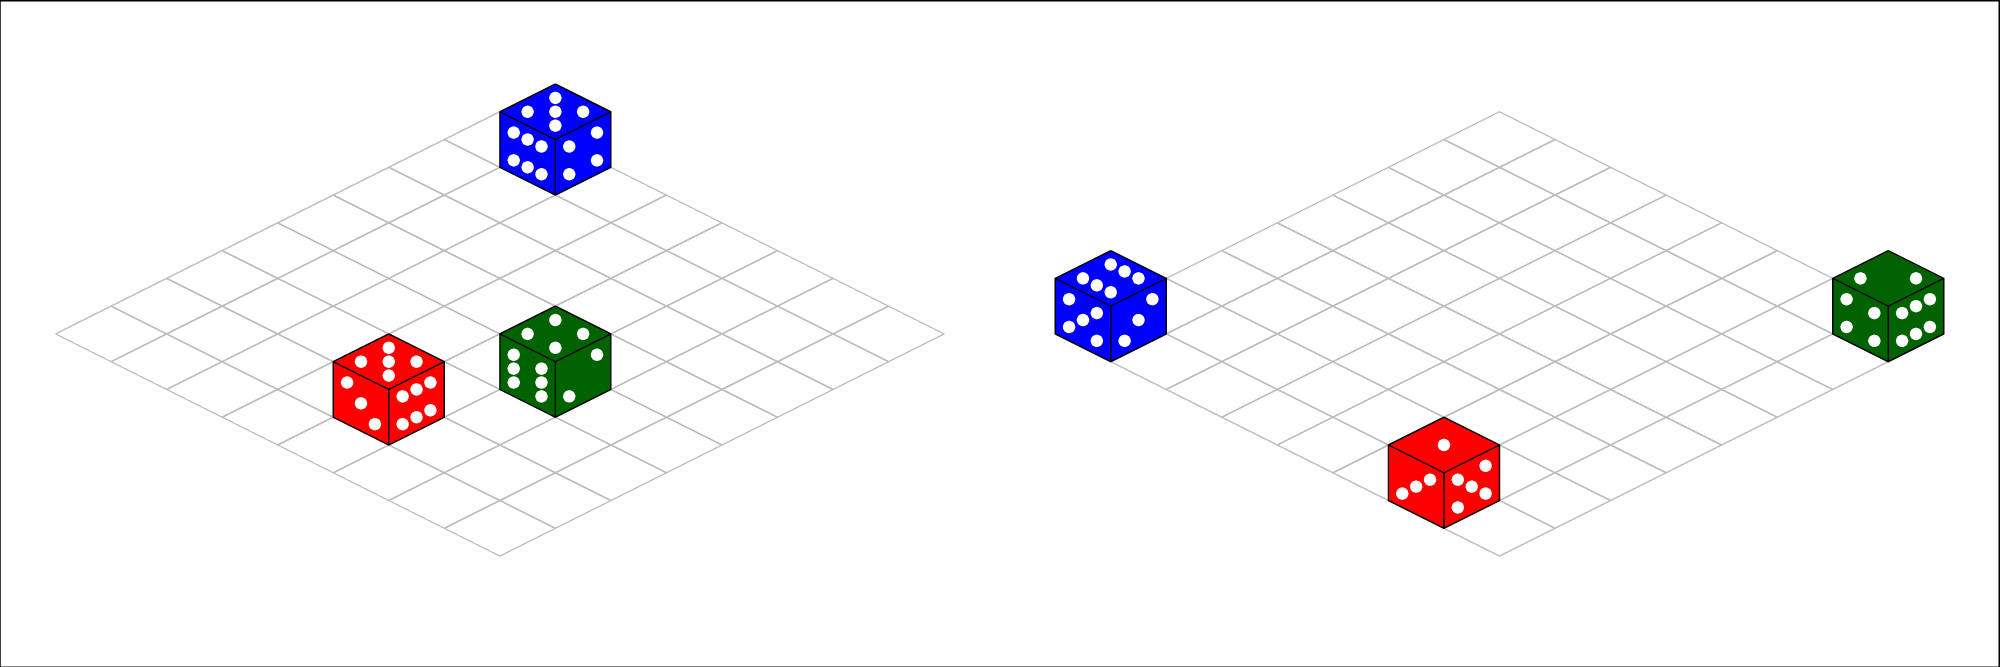
\includegraphics[width=0.8\linewidth]{diceBlue03.png}
      \\
      \textcolor{red}{DHER} |
      \textcolor{darkGreen}{URTI} |
      \textcolor{blue}{USTB}
    \end{tabular}
  \end{center}


  \newpage


  \begin{center}
    \begin{tabular}{c}
      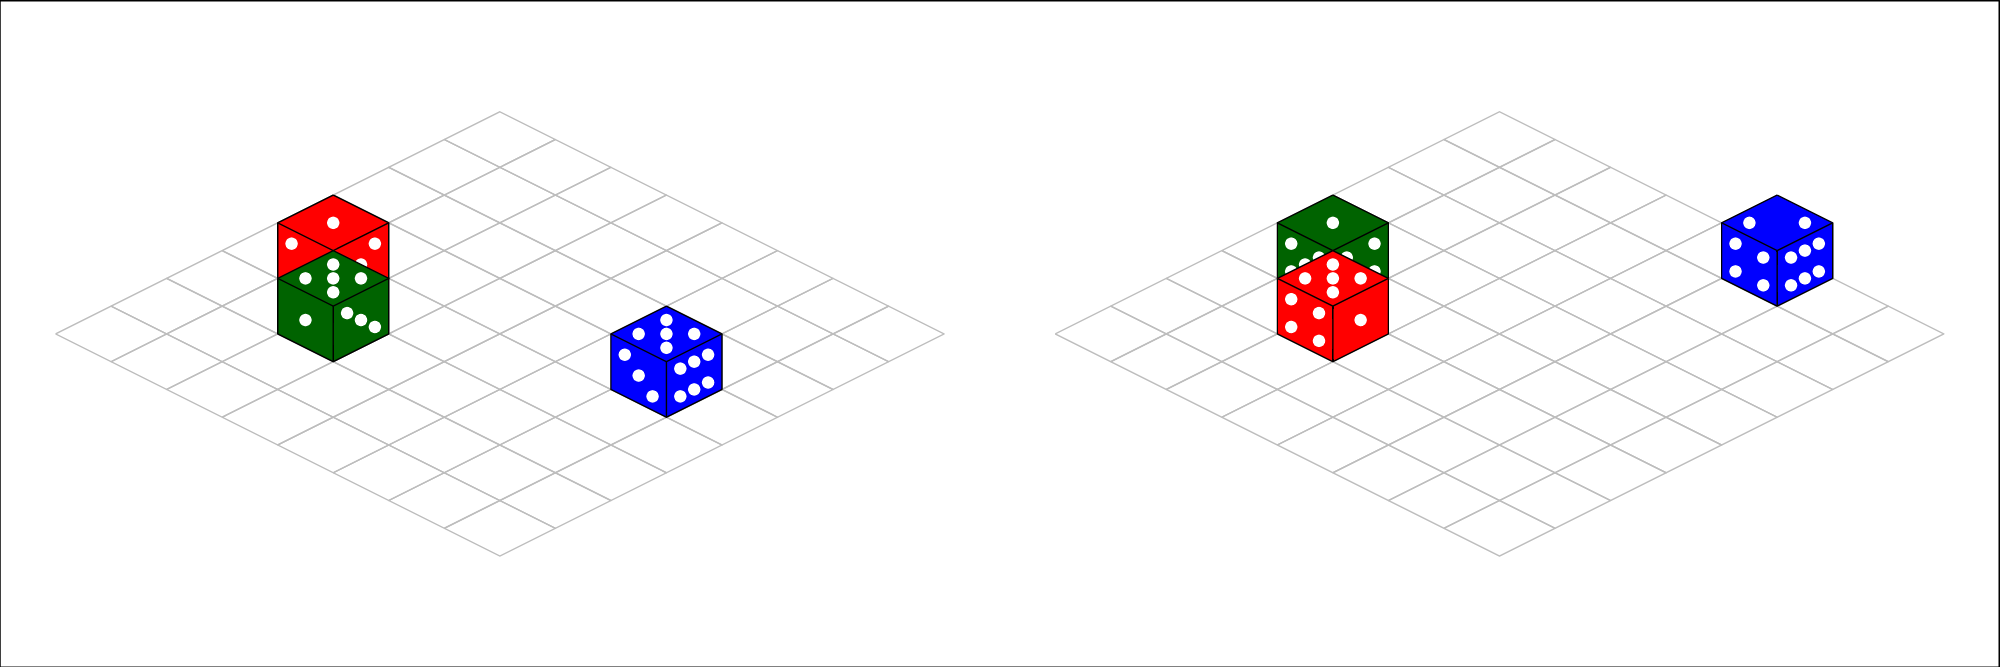
\includegraphics[width=0.8\linewidth]{diceGreen02.png}
      \\
      \textcolor{red}{MEO} |
      \textcolor{darkGreen}{LAC} |
      \textcolor{blue}{MEO}
    \end{tabular}
  \end{center}


  \vfill


  \begin{center}
    \begin{tabular}{c}
      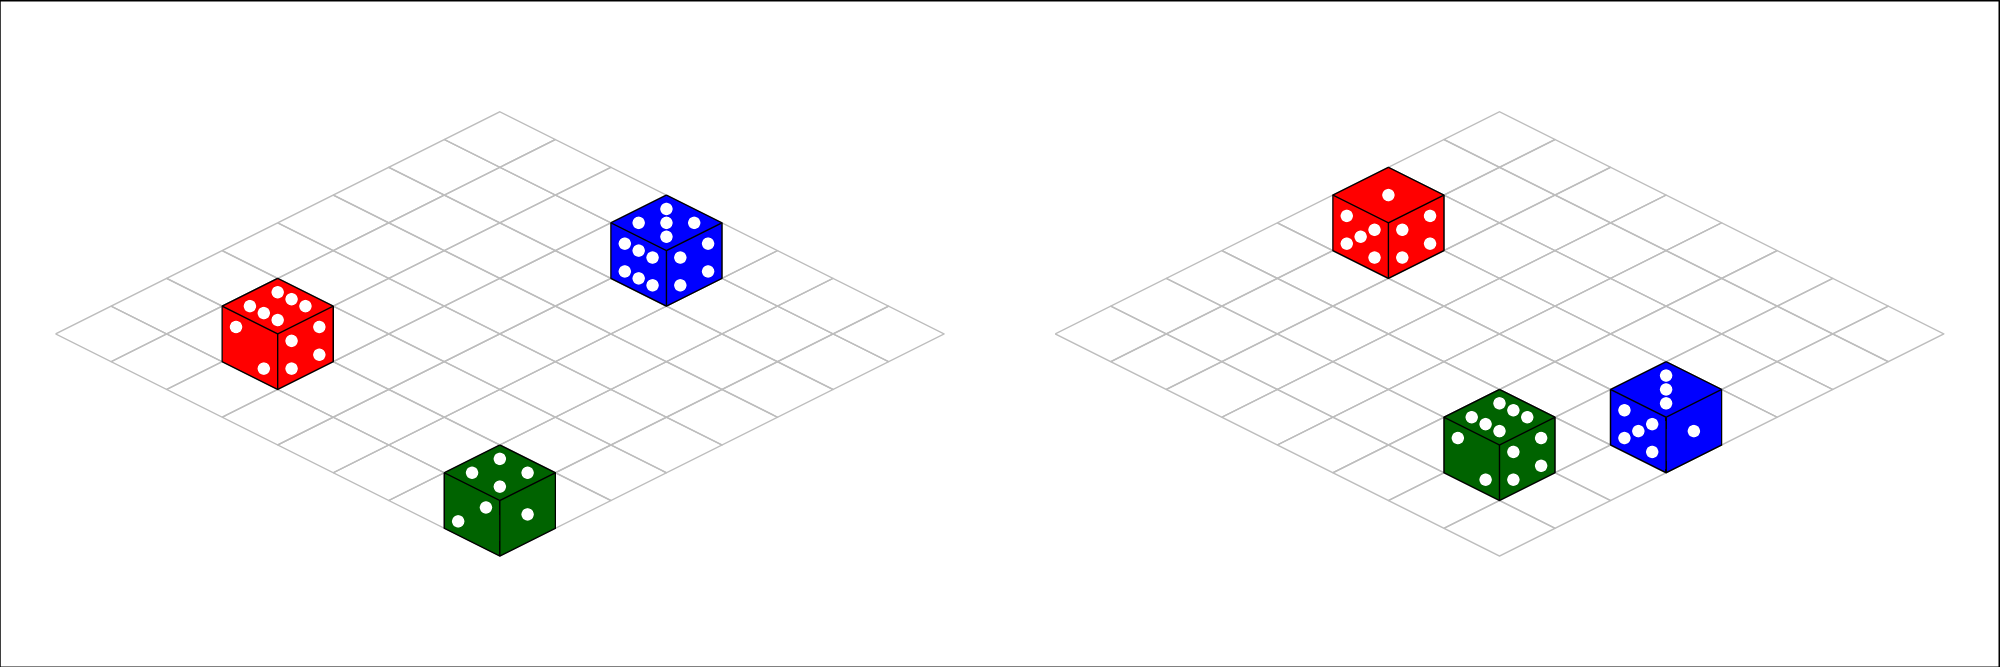
\includegraphics[width=0.8\linewidth]{diceGreen01.png}
      \\
      \textcolor{red}{YOU} |
      \textcolor{darkGreen}{REA} |
      \textcolor{blue}{YOU}
    \end{tabular}
  \end{center}


  \vfill


  \begin{center}
    \begin{tabular}{c}
      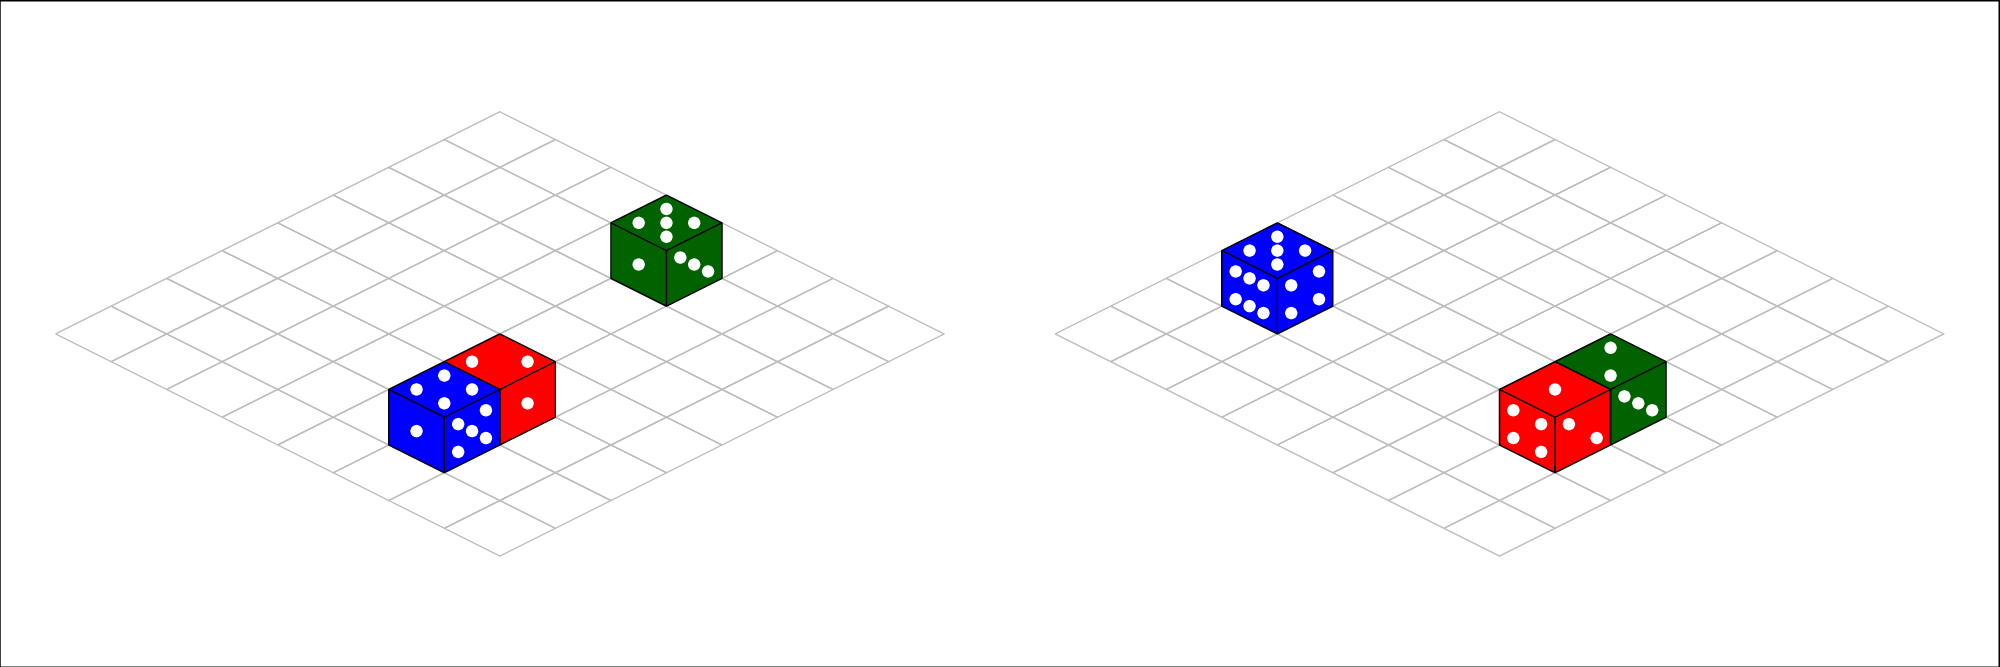
\includegraphics[width=0.8\linewidth]{diceGreen03.png}
      \\
      \textcolor{red}{ATH} |
      \textcolor{darkGreen}{ITE} |
      \textcolor{blue}{ATH}
    \end{tabular}
  \end{center}


  \newpage


  \begin{center}
    \begin{tabular}{c}
      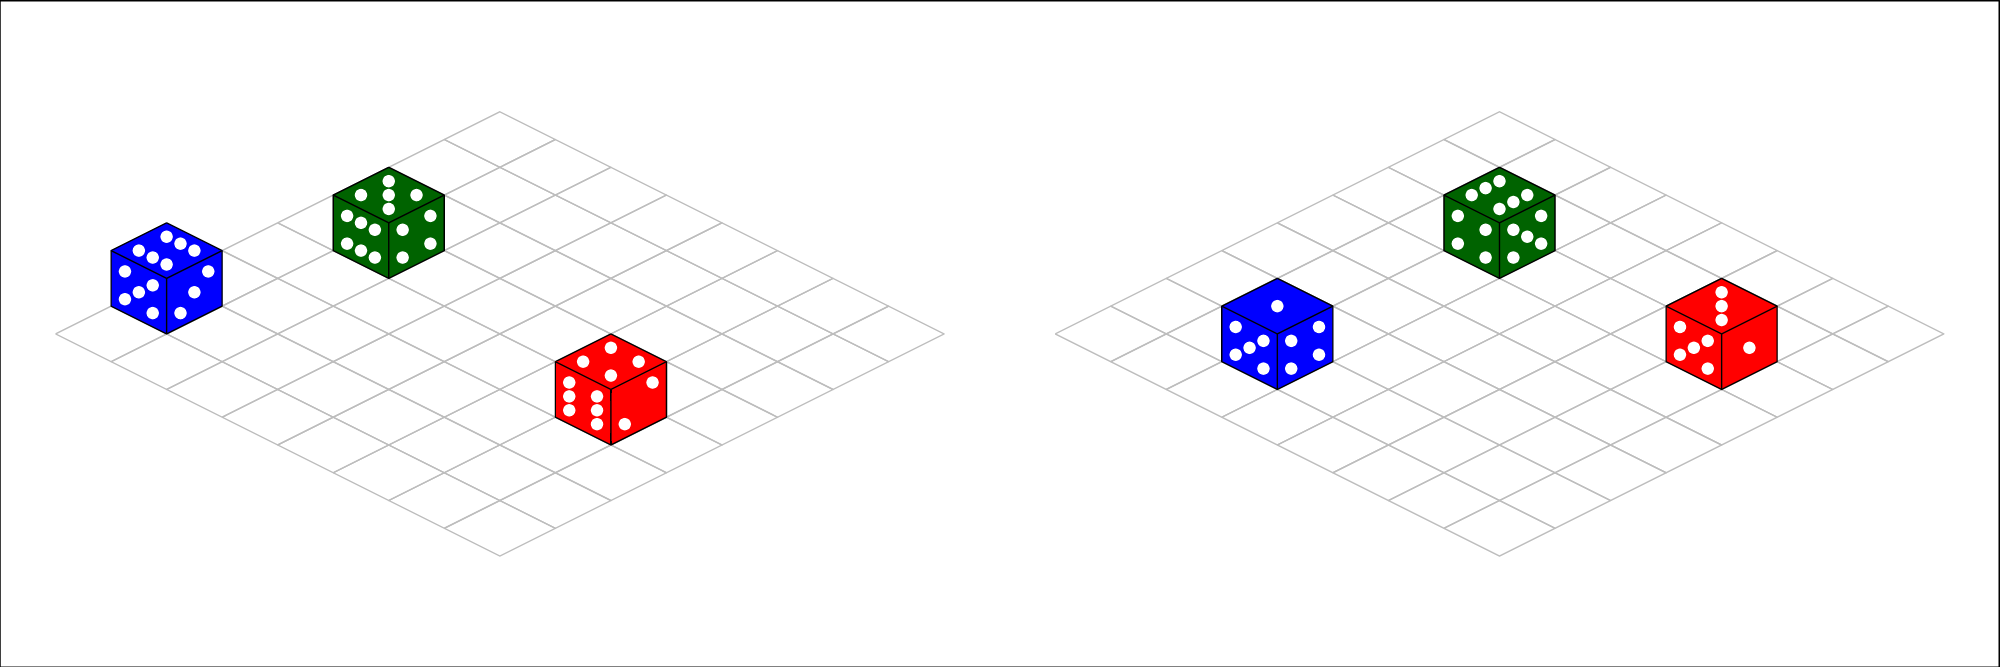
\includegraphics[width=0.8\linewidth]{diceRed02.png}
      \\
      \textcolor{red}{DIN} |
      \textcolor{darkGreen}{SIS} |
      \textcolor{blue}{VEW}
    \end{tabular}
  \end{center}


  \vfill


  \begin{center}
    \begin{tabular}{c}
      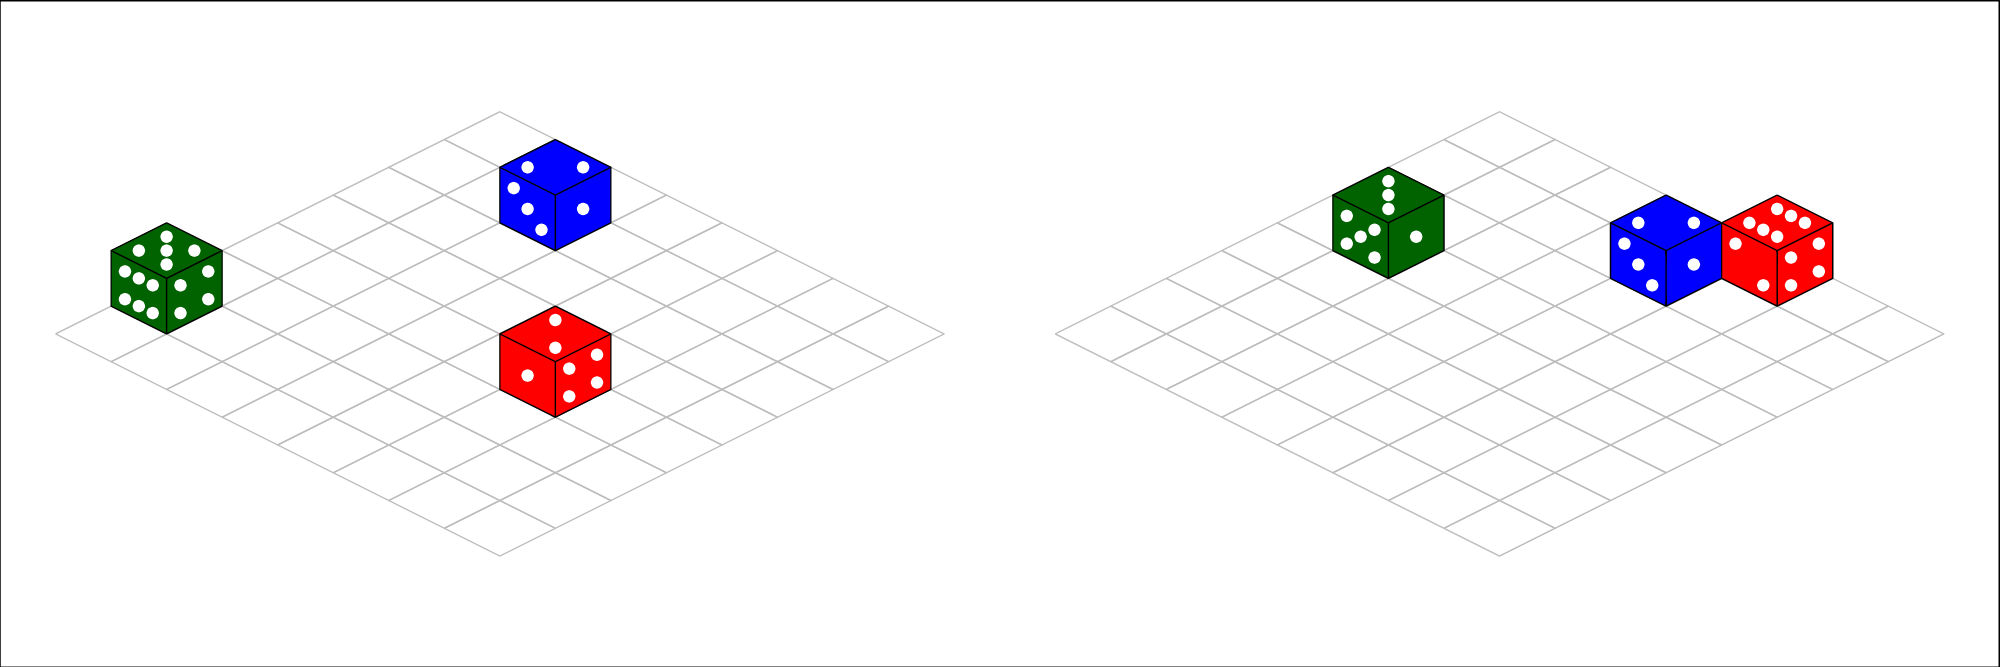
\includegraphics[width=0.8\linewidth]{diceRed01.png}
      \\
      \textcolor{red}{DWH} |
      \textcolor{darkGreen}{AFR} |
      \textcolor{blue}{ISP}
    \end{tabular}
  \end{center}


  \vfill


  \begin{center}
    \begin{tabular}{c}
      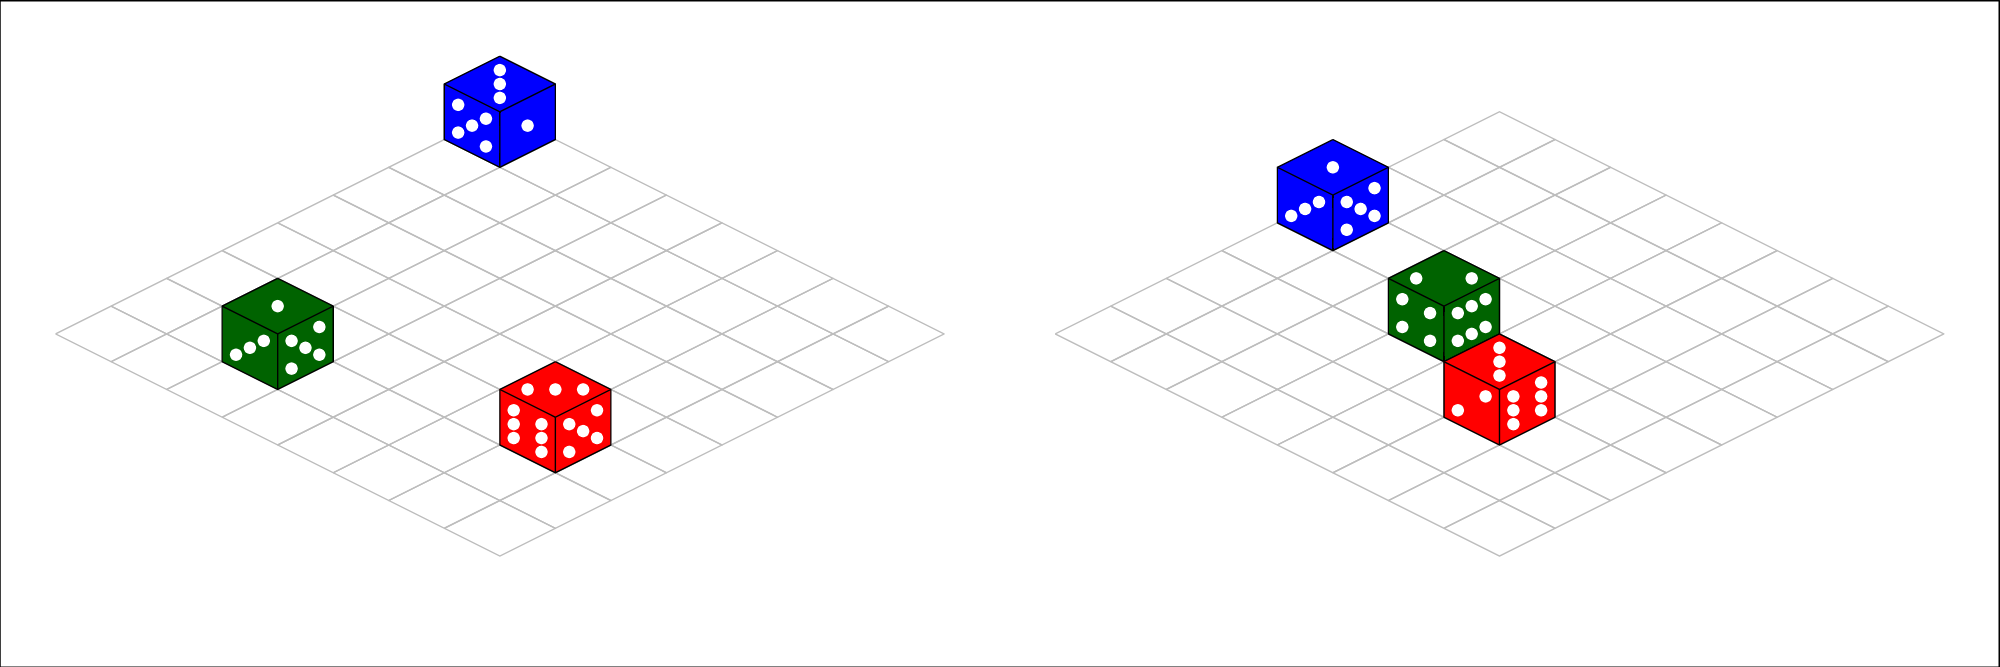
\includegraphics[width=0.8\linewidth]{diceBlue01.png}
      \\
      \textcolor{red}{GIM} |
      \textcolor{darkGreen}{NTH} |
      \textcolor{blue}{KAN}
    \end{tabular}
  \end{center}

\begin{center}
  \phLetterBox{}{}
  \phLetterBox{}{}
  \phLetterBox{}{}
  \phLetterBox{}{}
  \phLetterBox{}{}
  \phLetterBox{}{}
  \phLetterBox{}{}
  \phLetterBox{}{}
\end{center}
\begin{center}
  \phLetterBox{}{}
  \phLetterBox{}{}
  \phLetterBox{}{}
  \phLetterBox{}{}
  \phLetterBox{}{}
  \phLetterBox{}{}
  \phLetterBox{}{}
  \phLetterBox{}{}
\end{center}